\section{Aufgabe 6 - Motorsteuerung mit Nähreungssensor}
\label{sec:aufgabe-6---motorsteuerung-mit-naehreungssensor}

In dieser Aufgabe soll mithilfe ein Motor angesteuert werden.
Um die Geschwindigkeit des Motors zu steuern, wird eine Regulierung mittels PWM-Signal realisiert.
Der Motor soll weiters auf einen Ultraschallsensor reagieren, welche die Entfernung zu Objekten misst.
Nähert sich ein Objekt auf weniger als 30cm, so soll der Motor ausgeschaltet, bzw.\ seine Geschwindigkeit auf 0 reduziert, werden.
Eine 7-Segment Anzeige soll die derzeitige Geschwindigkeitsstufe des Motors anzeigen und mittels Schieberegister gesteuert werden.

Zwei Taster sollen einerseits die Laufrichtung des Motors und andererseits die Geschwindigkeit ändern.
Wird Taster A betätigt, soll sich die Geschwindigkeit, mit der sich der Motor gegen den Uhrzeigersinn dreht, um eins erhöht werden.
Dreht sich der Motor bei Betätigung des Tasters im Uhrzeigersinn, so wird die Laufrichtung und Geschwindikeit entsprechend geändert.
Wird Taster B gedrückt, soll das selbe Verhalten für die andere Laufrichtung implementiert werden.

Die Geschwindikeiten sollen hierbei zwischengespeichert und wiederhergestellt werden.
Es soll daher das folgende Beispiel möglich sein.

\begin{itemize}
    \item Motor dreht sich mit Geschwindigkeit 3 im Uhrzeigersinn
    \item Taster A wird betätigt
    \item Motor dreht sich mit Geschwindigkeit 1 gegen den Uhrzeigersinn
    \item Taster A wird betätigt
    \item Motor dreht sich mit Geschwindigkeit 2 gegen den Uhrzeigersinn
    \item Taster B wird betätigt
    \item Motor dreht sich mit Geschwindigkeit 4 im Uhrzeigersinn
    \item Taster B wird betätigt
    \item Motor dreht sich mit Geschwindigkeit 5 im Uhrzeigersinn
    \item Taster A wird betätigt
    \item Motor dreht sich mit Geschwindigkeit 3 gegen den Uhrzeigersinn
\end{itemize}

Würde die Geschwindigkeit mittels Tastendruck auf $> 9$ gebracht werden wird sie wieder auf 0 zurückgesetzt.

\subsection{Materialien}
\label{subsec:a6-materialien}

\begin{table}[h]
    \centering
    \caption{Aufgabe 6 - Verwendete Materialien}
    \label{tab:a6-materialien}
    \begin{tabular}{| l | l | l |}
        \hline
        Bezeichnung & Eigenschaften & Menge \\
        \hline
        7-Segement Anzeige & & 1 \\
        Ultraschallsensor & HC-SR04 & 1 \\
        Schieberegister & 74HC595 & 1 \\
        Taster & 4 Polig & 2\\
        Motortreiber & L293D & 1 \\
        LED & Rot & 1 \\
        LED & Grün & 1 \\
        Widerstand & $150\Omega$ & 10 \\
        & Braun - Grün - Braun - Gold & \\
        Widerstand & $10k\Omega$ & 2 \\
        & Braun - Schwarz - Orange - Gold & \\
        Diode & & 2 \\
        DC-Motor & & 1 \\
        Mikrocontroller & Arduino Uno R3 & 1 \\
        \hline
    \end{tabular}
\end{table}

\subsection{Vorbereitung}
\label{subsec:a6-vorbereitung}

\subsubsection{Aufgabe 1}
Als erste Aufgabe ist zu Überlegen, wie die Entfernungsmessung vorgenommen werden kann.
Dafür wird die Beschreibung des HC-SR04 Moduls von microcontroller.net verwendet \cite{ultraschallsensor}.

Es gibt für die Messung hierbei zwei Dinge zu berücksichtigen
Erstens, ein Messzyklus wird mit einer fallenden Flanke am Triggereingang gestartet.
Zweitens, das Ziel ist es, so oft wie möglich zu messen, da eine Sicherheitt gewährleistet werden soll.
D.h., der Motor soll ausschalten, da eine Gefährdung durch Nähe angenommen werden soll.
Daher muss ermittelt werden, wieviel ein Zeit eine Messung benötigt, um die Messabstände so kurz wie möglich zu machen.

Laut microcontroller.net kann ein 50Hz Rechtecksignal angelegt werden, um eine kontinuierliche Messung zu erreichen.
Es muss also alle 20ms eine fallende Flanke angelegt werden.
Eine fallende Flanke am Echo-Ausgang gibt dann an, dass das Echo des Ultraschallsignals gemessen wurde.
Mit der Dauer $t$ zwischen dem Start und Ende der Messung, sowie der Schallgeschwindigkeit in Luft $c_{Luft}=343,5\frac{m}{s}$, kann dann die Entfernung $d$ gemessen Werden.
Diese Dauer muss dann noch halbiert werden, da die gemessene Dauer den Hin- \textbf{und} Rückweg beinhaltet.

\begin{align}
    d = \frac{v * t}{2}
\end{align}


\subsubsection{Aufgabe 2}

Es sollen die Bytes gefunden werden, welche an das Schieberegister übertragen werden müssen, um die Zahlen von 1 bis 9 anzuzeigen.

\begin{table}
    \centering
    \caption{Aufgabe 6.2}
    \label{tab:aufgabe-6-2}
    \begin{tabular}{| l ||  l | l | l | l | l | l | l | l |}
        \hline
          & A & B & C & D & E & F & G & DP \\
        \hline
        0 & 1 & 1 & 1 & 1 & 1 & 1 & 0 & 0 \\
        1 & 0 & 1 & 1 & 0 & 0 & 0 & 0 & 0 \\
        2 & 1 & 1 & 0 & 1 & 1 & 0 & 1 & 0 \\
        3 & 1 & 1 & 1 & 1 & 0 & 0 & 1 & 0 \\
        4 & 0 & 1 & 1 & 0 & 0 & 1 & 1 & 0 \\
        5 & 1 & 0 & 1 & 1 & 0 & 1 & 1 & 0 \\
        6 & 1 & 0 & 1 & 1 & 1 & 1 & 1 & 0\\
        7 & 1 & 1 & 1 & 0 & 0 & 0 & 0 & 0 \\
        8 & 1 & 1 & 1 & 1 & 1 & 1 & 1 & 0 \\
        9 & 1 & 1 & 1 & 1 & 0 & 1 & 1 & 0 \\
        \hline
    \end{tabular}
\end{table}

\subsubsection{Aufgabe 3}

Wie in Sektion \ref{subsec:A1-vorbereitung} muss ein geeigneter Widerstand für die LEDs gefunden wernde.
Die Berechnung und des Widerstands und die reale Auswahl aus der E6-Reihe erfolgt wie in Sektion \ref{subsec:A1-vorbereitung}.
D.h., es wurden $200\Omega$ berechnet und der $150\Omega$ Widerstand aus der E6-Reihe ausgewählt.

\subsection{Praktikumsaufgabe}
\label{subsec:a6-praktikumsaufgabe}

Es wurde die Schaltung aus Abbildung \ref{fig:a6-implementierung} implementiert.
Für die Taster zur Geschwindigkeitssteuerung wurden die Pins 2 und 3 verwendet.
Des weiteren wurden sie, wie in Abschnitt \ref{sec:aufgabe-2---reaktionsspiel} als Pullup-Eingang konfiguriert und geschalten.

\begin{figure}[h]
    \centering
    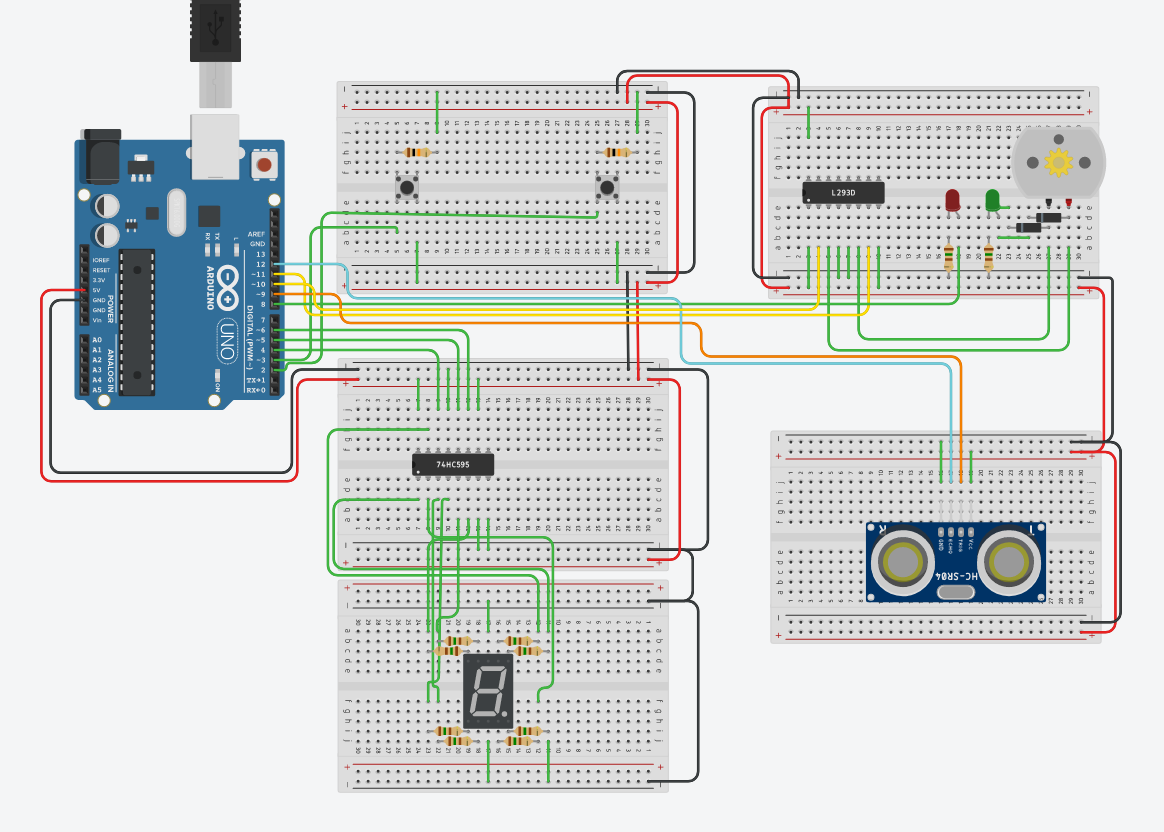
\includegraphics[width=\textwidth]{pictures/a6-praktikum.png}
    \caption{Implementierte Schaltung aus Aufgabe 6}
    \label{fig:a6-implementierung}
\end{figure}

Die Pins 4, 5 und 6 dienen der Steuerung des Schieberegisters.
Pin 5 dient dazu, den Schreibvorgang zu starten.
Ein $LOW$ Signal an diesem Pin führt dazu, dass Daten in das Schieberegister geschoben werden können.
Pin 4 legt das Datensignal an und Pin 6 dient zum synchronisieren des Datensignals mit den weiterschieben im Register.
D.h., an Pin 6 liegt das Clock-Signal an.

Die Ausgänge 1 bis 7 des Schieberegisters sind an den Eingängen A bis G der 7-Segment Anzeige angeschlossen.
Der Ausgang 8 sow der eingang $DP$ der 7-Segment Anzeige werden nicht benötigt und werden folglich an Masse angeschlossen.
Da die Anzeige aus LEDs besteht wird vor jedem Eingang ein Vorwiderstand von $150\Omega$ angeschlossen.

Die Pins 12 und 9 sind dem Ultraschallmodul angeschlossen.
Der Trigger Eingang wird von Pin 12 gesteuert.
Das Echo-Signal wird dann von Pin 9 empfangen.

Die Pins 11 und 10 werden für die Steuerung des Motors verwendet.
Um die Geschwindigkeit des Motors zu Steuern wird ein PWM-Signal verwendet, daher müssen auch die Pins ein PWM-Signal unterstüzen.
Der Motortreiber schaltet die Versogungsspannung dann entsprechend.
Je nach eingeschalteten Pin, 11 oder 10, dreht sich der Motor entweder nach Links oder nach Rechts.

Die Ausgänge des Motortreibers sind am Motor angeschlossen.
Eine Anforderung war, dass eine grüne LED leuchtet, wenn der Motor in Bewegung ist und eine Rote wenn er stoppt.
Um die Komplexität des Programms zu reduzieren, wurde die Funktion der grünen LED als Schaltung implementiert.
Zwei Dioden verbinden jeweils den Plus- und Minuspol des Motors mit der LED.
Die Dioden werden benötigt um einen Strom in Richtung Motor zu unterbinden.
Die LED leuchtet dann immer, wenn eine Spannung am Motor anliegt.
Da der Motor mittels PWM gesteuert wird, leuchtet die LED stärker, je schneller der Motor läuft.
Die rote LED wird mittel Pin 8 gesteuert.

Im nachfolgenden Text wird der Programmcode der Aufgabe erläutert.
Einzelne Teile des Codes werden ausgewählt und beschrieben.
Am Ende dieser Sektion befindet sich der vollständige Programmcode.

\begin{lstlisting}[language=C,label={lst:a6-segment-konstanten}, caption={Wichtige Konstanten}]
const int SEGMENT_COUNT = 10;

const int DELAY_TRIGGER = 20;
const int DELAY_READ = 550;

const byte MAX_MOTOR_SPEED = 255;
const byte SEGMENT_DISPLAY[] = {
B11111100,
B01100000,
B11011010,
B11110010,
B01100110,
B10110110,
B10111110,
B11100000,
B11111110,
B11110110
};
\end{lstlisting}

In Listing \ref{lst:a6-segment-konstanten} sind wichtige Konstanten enthalten.
$SEGMENT\_DISPLAY$ ist ein Array, welches die Bytes enthält, die zum Anzeigen der Zahlen von 0 bis 9 benötigt wird.
$SEGMENT\_COUNT$ beinhaltet die Länge des Arrays.
Die Werte für $SEGMENT\_DISPLAY$ wurde aus Aufgabe 2 der Sektion \ref{subsec:a6-vorbereitung} entnommen.
Der Wert $DELAY\_TRIGGER$ wird verwendet, um die Steuerung des Ultraschallsensors zu timen.
Um die Geschwindigkeit pro Geschwindigkeitsstufe zu errechnen, wird später im Programm die Konstante $MAX\_MOTOR\_SPEED$ verwendet.


\begin{lstlisting}[language=C,label={lst:a6-variablen}, caption={Wichtige Variablen}]
volatile int segment_index_left = 0;
volatile int segment_index_right = 0;

/*
true => motor turns right,
false => motor turns left
*/
volatile bool turn_direction = true;
\end{lstlisting}

Die in Listing \ref{lst:a6-variablen} gezeigten Variablen $segment\_index\_left$ und $segment\_index\_right$ werden verwendet, um die Geschwindigkeit nach Links, bzw.\ nach Rechts, des Motors zu speichern.
$turn\_direction$ gibt an, ob sich der Motor nach Rechts oder nach Links derehen soll.
Ist die Variable auf $true$ gesetzt, soll sich der Motor nach Rechts drehen, ansonsten nach Links.
Alle drei Variablen besitzen das $volatile$ Schlüsselwort, da sie von Interrupts beschrieben und gelesen werden.

\begin{lstlisting}[language=C,label={lst:a6-setup-taster}, caption={Setup der Taster}]
setup() {
    ...

    attachInterrupt(
    digitalPinToInterrupt(PIN_BUTTON_LEFT),
    on_button_left_rising,
    RISING);

    attachInterrupt(
    digitalPinToInterrupt(PIN_BUTTON_RIGHT),
    on_button_right_rising,
    RISING);

    ...
}
\end{lstlisting}

In Listing \ref{lst:a6-setup-taster} werden die Taster mit Interrupts verknüpft.
Anders als in Abschnitt \ref{sec:aufgabe-2---reaktionsspiel}, wird nur ein Interrupt beim Drücken des Tasters benötigt, nicht jedoch beim los lassen.
Daher wird der $attachInterrupt(\dots)$ Methode lediglich $RISING$ anstatt $CHANGE$ mitgegeben.

\begin{lstlisting}[language=C,label={lst:a6-interrupts}, caption={Interrupts der Taster}]
void on_button_left_rising() {
    segment_index_left++;

    if (segment_index_left >= SEGMENT_COUNT) {
        segment_index_left = 0;
    }
    turn_direction = false;
}

void on_button_right_rising() {
    segment_index_right++;

    if (segment_index_right >= SEGMENT_COUNT) {
        segment_index_right = 0;
    }
    turn_direction = true;
}
\end{lstlisting}

Die verknüpften Interrupts sind in Listing \ref{lst:a6-interrupts} zu sehen.
Beide sind analog zueinander im Bezug auf die Drehrichtung des Motors.
Wird ein Taster betätigt, wird zuerst die $segment\_index\_*$ Variable erhöht.
Übersteigt diese die Anzahl an Indices des $SEGMENT\_DISPLAY$ Arrays, wird sie auf 0 zurückgesetzt.
Abschließend wird die Variable zur Steuerung der Drehrichtung entsprechend gesetzt.

\begin{lstlisting}[language=C,label={lst:a6-update-display}, caption={Aktualisierung der 7-Segment-Anzeige}]
void update_display(byte value)
{
    digitalWrite(PIN_LATCH, LOW);
    shiftOut(PIN_DATA, PIN_CLOCK, LSBFIRST, value);
    digitalWrite(PIN_LATCH, HIGH);
}
\end{lstlisting}

In Listing \ref{lst:a6-update-display} wird die 7-Segment-Anzeige auf den übergebenen Wert aktualisiert.
Dafür wird zuerst Pin 5, welcher den Schreibzugriff regelt, auf $LOW$ geschalten.
Damit ist das Schieberegister bereit zum beschrieben werden.
Die Methode $shiftOut(\dots)$ schreibt dann, unter verwendung des Daten- und Clockpins, den Wert in das Register.
Anschließend wird mit dem Setzen auf $HIGH$ des Pin 5 das Schreiben beendet.

\begin{lstlisting}[language=C,label={lst:a6-distanz-messung}, caption={Distanz Messung}]
bool is_distance_safe() {
    // Clear trigger
    digitalWrite(PIN_ULTRASONIC_TRIGGER, LOW);
    delayMicroseconds(DELAY_TRIGGER);

    // Send High Signal
    digitalWrite(PIN_ULTRASONIC_TRIGGER, HIGH);
    delayMicroseconds(DELAY_TRIGGER);
    digitalWrite(PIN_ULTRASONIC_TRIGGER, LOW);

    double duration = pulseIn(PIN_ULTRASONIC_ECHO, HIGH);
    double distance= duration*0.034/2;

    return distance > 30;
}
\end{lstlisting}

Die Messung der Distanz wird in Listing \ref{lst:a6-distanz-messung} durchgeführt.
Der Trigger wird dazu zuerst auf für 20ms auf $LOW$ geschalten um einen konsistenten Zustand zu erreichen.
Dannach wird der Messvorgang gestartet, indem der Trigger für 20ms auf $HIGH$ geschalten wird und anschließend wieder auf $LOW$.
Durch $pulseIn(\dots)$ blockiert das Programm, bis ein Signal am Echo-Pin anliegt und gibt dann die vergangene Zeit, in Mikrosekunden, zurück.
Die Distanz beträgt dann:

\begin{align}
    d = \frac{t[\mu s] * 343 \frac{m}{\mathbf{s}}}{2} \\
    = \frac{t[\mu s] * 0.000343 \frac{m}{\mathbf{\mu s}}}{2} \\
    = \frac{t[\mu s] * 0.0343 \frac{\mathbf{cm}}{\mu s}}{2}
\end{align}

Da der Sicherheitsabstand 30cm beträgt, wird wahr, bzw.\ $true$, zurückgegeben, wenn der Abstand $> 30cm$ ist, ansonsten falsch, bzw.\ $false$.

\begin{lstlisting}[language=C,label={lst:a6-aktualisieren-7-segment-anzeige}, caption={Einstellen der 7-Segment Anzeige}]
void loop()
{
    int segment_index = 0;

    if (turn_direction) {
    segment_index = segment_index_right;
    } else {
    segment_index = segment_index_left;
    }

    update_display(SEGMENT_DISPLAY[segment_index]);

    ...
\end{lstlisting}

Zuerst wird in Listing \ref{lst:a6-aktualisieren-7-segment-anzeige}, je nach Drehrichtung, die enstprechende $segment\_index\_*$ Variable in $segment\_index$ gespeichert.
Der zugehörige Wert des $SEGMENT\_DISPLAY$ Arrays wird dann der $update\_display$ Methode übergeben.
Dadurch wird die aktuelle Geschwindigkeit des Motors angezeigt.

\begin{lstlisting}[language=C,label={lst:a6-moto-geschwindigkeit-berechnen}, caption={Berechnung des PWM-Signals}]
    ...

    byte motor_speed = MAX_MOTOR_SPEED
        / SEGMENT_COUNT
        * segment_index;

    if (!is_distance_safe()) {
        motor_speed = 0;
    }

    ...
\end{lstlisting}

Die ''Stärke'' des PWM-Signals wird nun in Listing \ref{lst:a6-moto-geschwindigkeit-berechnen} berechnet.
Eine Division der $MAX\_MOTOR\_SPEED$ Konstanten durch die Anzahl an Geschwindigkeitsstufen wird durchgeführt und dann mit der aktuellen Geschwindigkeit multipliziert.
Dadurch ergibt sich der Wert, auf den das PWM-Signal eingestellt werden muss.
Sollte es sich herausstellen, dass der Sicherheitsabstand unterschritten wird, wird der Wert auf 0 gesetzt.

\begin{lstlisting}[language=C,label={lst:a6-motor-steuerung}, caption={Ansteuerung des Motors}]
    ...

    if (turn_direction) {
        analogWrite(PIN_MOTOR_RIGHT, motor_speed);
        analogWrite(PIN_MOTOR_LEFT, 0);
    } else {
        analogWrite(PIN_MOTOR_LEFT, motor_speed);
        analogWrite(PIN_MOTOR_RIGHT, 0);
    }

    if (motor_speed > 0) {
        digitalWrite(PIN_STOP_LED, LOW);
    } else {
        digitalWrite(PIN_STOP_LED, HIGH);
    }

    ...
\end{lstlisting}

Unter Verwendung der $analogWrite(\dots)$ Methode wird nun das PWM-Signal ausgegeben.
Dieser Vorgang ist in Listing \ref{lst:a6-motor-steuerung} abgebildet.
Je nach Drehrichtung wird das Signal entweder an Pin 12 oder 10 angelegt.
Der jeweils andere Pin wird ausgeschaltet.
Abschließend wird die rote LED ausgeschaltet, wenn die Geschwindigkeit $> 0$ beträgt, oder eingeschalten, wenn dies nicht der Fall ist.

\begin{lstlisting}[language=C,label={lst:a6-programmcode}, caption={Vollständiger Programmcode der Aufgabe 6}]
/*
Adafruit Arduino - Lesson 4. 8 LEDs and a Shift Register
*/

const int PIN_LATCH = 5;
const int PIN_CLOCK = 6;
const int PIN_DATA = 4;
const int PIN_MOTOR_LEFT = 11;
const int PIN_MOTOR_RIGHT = 10;
const int PIN_STOP_LED = 8;

const int PIN_BUTTON_LEFT = 3;
const int PIN_BUTTON_RIGHT = 2;
const int PIN_ULTRASONIC_TRIGGER = 9;
const int PIN_ULTRASONIC_ECHO = 12;

const int SEGMENT_COUNT = 10;

const int DELAY_TRIGGER = 20;
const int DELAY_READ = 550;

const byte MAX_MOTOR_SPEED = 255;
const byte SEGMENT_DISPLAY[] = {
  B11111100,
  B01100000,
  B11011010,
  B11110010,
  B01100110,
  B10110110,
  B10111110,
  B11100000,
  B11111110,
  B11110110
};


volatile int segment_index_left = 0;
volatile int segment_index_right = 0;

/*
true => motor turns right,
false => motor turns left
*/
volatile bool turn_direction = true;

unsigned long previous_time = 0;

void setup()
{
  Serial.begin(115000);

  pinMode(PIN_LATCH, OUTPUT);
  pinMode(PIN_DATA, OUTPUT);
  pinMode(PIN_CLOCK, OUTPUT);
  pinMode(PIN_MOTOR_LEFT, OUTPUT);
  pinMode(PIN_MOTOR_RIGHT, OUTPUT);
  pinMode(PIN_STOP_LED, OUTPUT);

  pinMode(PIN_ULTRASONIC_TRIGGER, OUTPUT);
  pinMode(PIN_ULTRASONIC_ECHO, INPUT);

  pinMode(PIN_BUTTON_LEFT, INPUT_PULLUP);
  pinMode(PIN_BUTTON_RIGHT, INPUT_PULLUP);

  attachInterrupt(
    digitalPinToInterrupt(PIN_BUTTON_LEFT),
    on_button_left_rising,
    RISING);

  attachInterrupt(
    digitalPinToInterrupt(PIN_BUTTON_RIGHT),
    on_button_right_rising,
    RISING);

  digitalWrite(PIN_ULTRASONIC_TRIGGER, HIGH);
}

void loop()
{
  int segment_index = 0;

  if (turn_direction) {
    segment_index = segment_index_right;
  } else {
    segment_index = segment_index_left;
  }

  update_display(SEGMENT_DISPLAY[segment_index]);

  byte motor_speed = MAX_MOTOR_SPEED
    / SEGMENT_COUNT
    * segment_index;

  if (!is_distance_safe()) {
    motor_speed = 0;
  }

  if (turn_direction) {
    analogWrite(PIN_MOTOR_RIGHT, motor_speed);
    analogWrite(PIN_MOTOR_LEFT, 0);
  } else {
    analogWrite(PIN_MOTOR_LEFT, motor_speed);
    analogWrite(PIN_MOTOR_RIGHT, 0);
  }

  if (motor_speed > 0) {
    digitalWrite(PIN_STOP_LED, LOW);
  } else {
    digitalWrite(PIN_STOP_LED, HIGH);
  }
}

bool is_distance_safe() {
  // Clear trigger
  digitalWrite(PIN_ULTRASONIC_TRIGGER, LOW);
  delayMicroseconds(DELAY_TRIGGER);

  // Send High Signal
  digitalWrite(PIN_ULTRASONIC_TRIGGER, HIGH);
  delayMicroseconds(DELAY_TRIGGER);
  digitalWrite(PIN_ULTRASONIC_TRIGGER, LOW);

  double duration = pulseIn(PIN_ULTRASONIC_ECHO, HIGH);
  double distance= duration*0.034/2;

  return distance > 30;
}

void update_display(byte value)
{
   digitalWrite(PIN_LATCH, LOW);
   shiftOut(PIN_DATA, PIN_CLOCK, LSBFIRST, value);
   digitalWrite(PIN_LATCH, HIGH);
}

void on_button_left_rising() {
  segment_index_left++;

  if (segment_index_left >= SEGMENT_COUNT) {
    segment_index_left = 0;
  }
  turn_direction = false;
}

void on_button_right_rising() {
  segment_index_right++;

  if (segment_index_right >= SEGMENT_COUNT) {
    segment_index_right = 0;
  }
  turn_direction = true;
}
\end{lstlisting}

\subsection{Fehlerdiskussion}
\label{subsec:a6-fehlerdiskussion}

Die Konstante $DELAY\_READ$ wird nicht verwendet und ist ein Artefakt aus der Entwicklung des Programms.
Sie kann ohne Konsequenzen gelöscht werden.

Der Strom durch das Schieberegister bei eingeschalteter Anzeige ist zu hoch.
Eine andere Wahl der Widerstände würde dies verhinder.
Nach Experimentieren an der Schaltung stellt sich heraus, dass ein Widerstand von $500\Omega$ zu akzeptablen Resultaten führt.

\subsection{Zusammenfassung}
\label{subsec:a6-zusammenfassung}
